\todo{Opis implementacji systemu}

Przygotowany system odpowiadania na pytania został zaprojektowany w~oparciu o~modularne mikrousługi, komunikujące się ze sobą wykorzystując REST API. Takie podejście pozwoliło nam wykorzystać zewnętrzne usługi, oferujące narzędzia do przetwarzania języka naturalnego, bez ich instalacji na lokalnej maszynach. Zastosowanie architektury mikroserwisowej pozwala również na prostsze skalowanie rozwiązania oraz łatwiejsze udostępnianie systemu w~sieci WWW.

\begin{figure}[h]
    \centering
    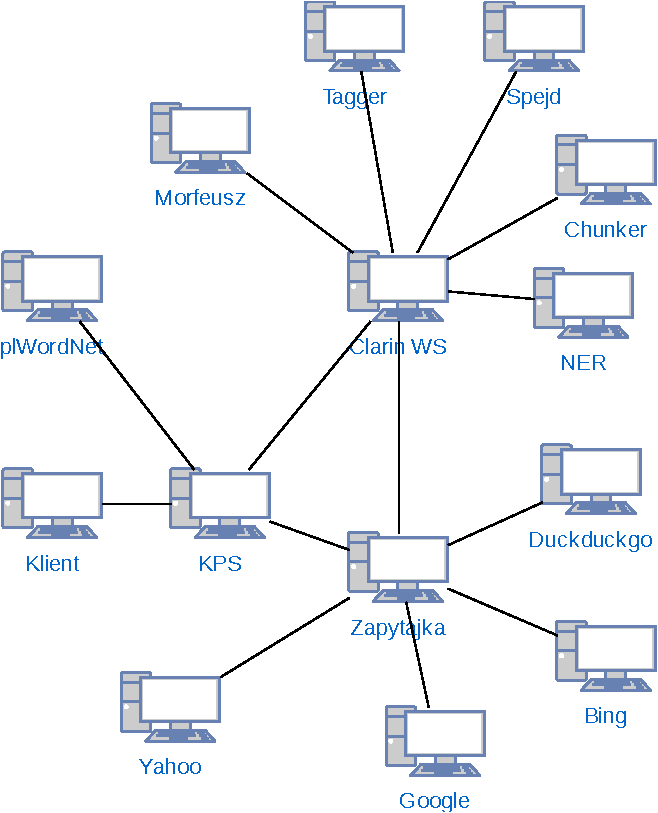
\includegraphics[width=\columnwidth]{figures/WEDT-Uslugi.pdf}
    \caption{Ogólny schemat komunikacji pomiędzy mikrousługami w~systemie}
    \label{fig:microservices}
\end{figure}

Na rysunku~\ref{fig:microservices} przedstawiony został ogólny schemat komunikacji pomiędzy poszczególnymi usługami. Centralną częścią systemu jest moduł \texttt{KPS}. Jego rolą jest zlecanie zadań innym usługom, analiza zwróconych przez nie wyników, a przede wszystkim odpowiadanie na pytania. Został on w~całości napisany w~języku Python, wykorzystując do komunikacji bibliotekę \texttt{Flask}.

Zadawanie pytań odbywa się przy użyciu aplikacji klienckiej. Dzięki temu że moduł \texttt{KPS} wystawia REST API umożliwiające odpytywanie, aplikacją kliencką może być każdy program, który jest w~stanie obsługiwać gniazda BSD oraz wiadomości w~formacie JSON. Do normalnego użytku, moduł \texttt{KPS} udostępnia prostą aplikację kliencką możliwą do uruchomienia z~poziomu przeglądarki, natomiast do automatycznego testowania, wykorzystany został skrypt w~języku Python. \todo{opisać implementacje pakietu algorithm, klasy i powiazania}

Drugim kluczowym modułem, który został w~całości przygotowany przez nasz zespół, był moduł \texttt{Zapytajka}. Jego rolą w~systemie jest agregacja podsumowań z~czterech różnych wyszukiwarek internetowych. Spełnia on rolę interfejsu pomiędzy aplikacją IR a~siecią~WWW. Moduł ten, podobnie jak poprzedni, został przygotowany przy pomocy języka Python i~biblioteki \texttt{Flask}. Moduł ten udostępnia proste REST API do komunikacji \textit{proces-proces} oraz prosty interfejs graficzny do komunikacji \textit{człowiek-proces}.

Moduł \texttt{Zapytajka} do zbierania podsumowań wykorzystuje silnik Selenium. Z~powodu iż wszystkie cztery omawiane wyszukiwarki nie udostępniają prostego, a~w~szczególności darmowego API do odpytywania ich silnika, w~naszym rozwiązaniu korzystamy z~procesu \textit{webscrapingu}, czyli renderowania pobranej strony w~przeglądarce, a~następnie analizie otrzymanego dokumentu HTML, filtracji niepotrzebnych tagów i ekstrakcji szukanych fragmentów. Rozwiązanie to nie jest pozbawione wad, producenci wyszukiwarek na bieżąco zmieniają układ dokumentu HTML, tak aby uniemożliwić zbyt intensywne \textit{webscrapowanie}, dlatego też ważne jest aby stale utrzymywać kod tego modułu i na bieżąco go modyfikować.

W~momencie przyjścia pytania, na które moduł ma znaleźć potencjalne odpowiedzi, uruchamiany jest nowy proces przeglądarki Firefox. W~międzyczasie, pytanie przekazywane jest do modułu generacji zapytań. Moduł ten na podstawie przekazanego parametru, wybiera algorytm generacji nowych zapytań na podstawie oryginalnego pytania.
Zaimplementowane zostały trzy strategię:
\begin{itemize}
    \item singlequery -- brak modyfikacji oryginalnego zapytania,
    \item stopwords -- usunięcie z~zapytania tak zwanych \textit{stopwordów} w~celu zwiększenia gęstości informacji,
    \item chunks -- podział pytania na kilka powiązanych wewnętrznie fraz (chunków), z~wykorzystaniem narzędzia \textit{iobber}.
\end{itemize}
Dzięki zastosowaniu wzorca \textit{dependency injection}, rozwiązanie to jest w~bardzo prosty sposób rozszerzalne o~nowe strategię generacji zapytań. 

Przedstawione do tej pory moduły zostały w~całości przygotowane przez nasz zespół. Pozostałe usługi wykorzystywane w~systemie, zostały publicznie udostępnione i znalezione przez nas w~internecie. Najważniejszą z~nich jest usługa CLARIN, udostępniająca poszczególne narzędzia do przetwarzania języka naturalnego, również w~języku polskim. CLARIN to europejska sieć badawcza zajmująca się archiwizacją i przetwarzaniem zasobów językowych w naukach humanistycznych i społecznych. CLARIN to skrót od Common Language Resources and Technology Infrastructure.

Wykorzystując ogólnie dostępne REST API z~systemu CLARIN, nasz system wykorzystuje takie narzędzia jak:
\begin{itemize}
    \item analizator morfologiczny \textit{morfeusz},
    \item tagger \textit{morfoDita},
    \item narzędzie do NER \textit{liner2},
    \item parser składniowy \textit{spejd},
    \item chunker \textit{iobber}.
\end{itemize}

Oprócz systemu CLARIN, nasze rozwiązanie wykorzystywało również REST API udostępnione przez usługę \textit{plWordNet}, służącą do zamiany słów na odpowiadające im lemmy.

Integracja z~zewnętrznymi systemami została zrealizowana za pomocą specjalnie przygotowanych interfejsów dostępowych, zagregowanych w~jeden pakiet języka \texttt{Python} nazwany \texttt{services}. W~skład tego pakietu wchodzą klasy służące do komunikacji z~usługami zewnętrznymi oraz wyszukiwarkami internetowymi. Na rysunku~\ref{fig:services-classes} przedstawiony został diagram klas, który przedstawia jakie klasy zawiera ten pakiet oraz jakie relacje występują pomiędzy nimi.

\begin{figure}[h]
    \centering
    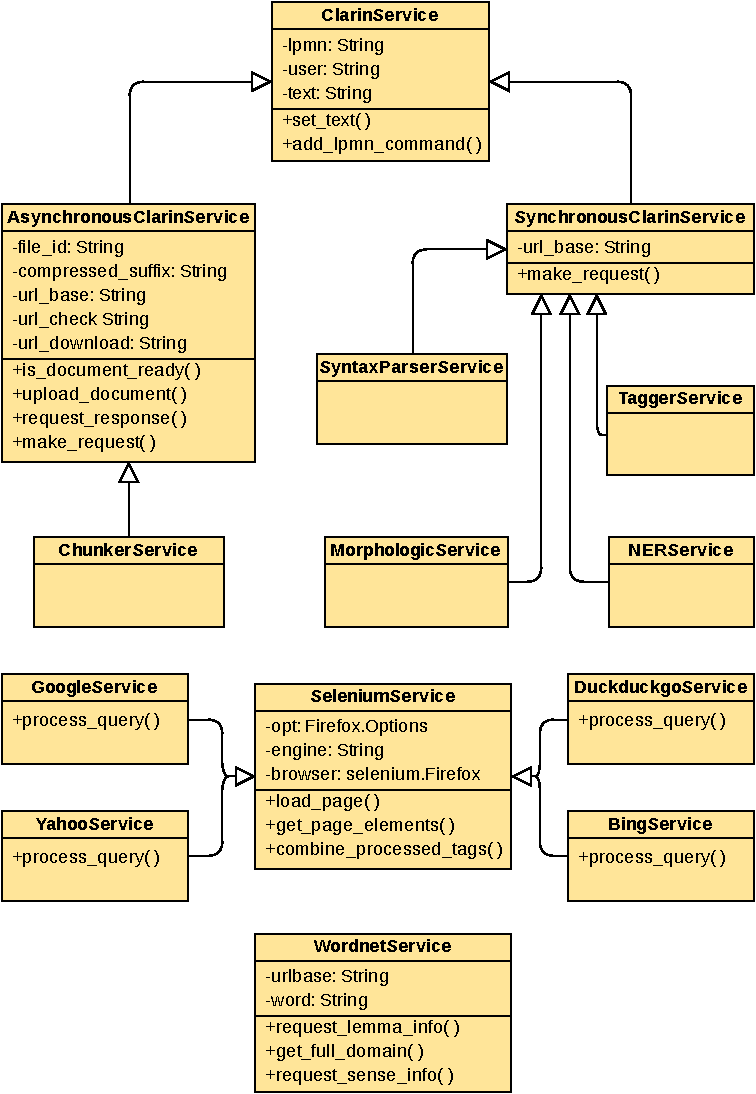
\includegraphics[width=\columnwidth]{figures/WEDT-Klasy.pdf}
    \caption{Diagram klas pakietu \texttt{services}}
    \label{fig:services-classes}
\end{figure}